\documentclass[12pt, a4paper]{article}

\usepackage{fancyhdr}
\usepackage[left=4cm, right=4cm, top=4cm, bottom=4cm]{geometry}
\usepackage[utf8]{inputenc}
\usepackage[table]{xcolor}
\usepackage{hyperref}
\usepackage{amsmath}
\usepackage{enumitem}
\usepackage{graphicx}
\usepackage{booktabs}
\usepackage{subcaption}
\usepackage[justification=centering]{caption}
\usepackage{xepersian}

\DeclareMathOperator*{\argmax}{argmax}
\DeclareMathOperator*{\argmin}{argmin}
\newcolumntype{L}{>{$}l<{$}} % math-mode version of "l" column type

\newcommand{\coursetitle}{شبکه‌های عصبی}
\newcommand{\doctitle}{تمرین پنجم}
\newcommand{\name}{محمدرضا غفرانی}
\newcommand{\studentno}{400131076}
\newcommand{\todaydate}{\today}

\settextfont{XB Kayhan}
\setlatintextfont{Times Newer Roman}

\pagestyle{fancy}
\lhead{\textbf{\doctitle}}
\chead{\name}
\rhead{\todaydate}

\begin{document}

\begin{flushleft}
    \name \\
    \studentno \\
    \todaydate
\end{flushleft}

\begin{center}
    \huge
    \textbf{\coursetitle}
    \break
    \large
    \doctitle
\end{center}

% suppress the fancy header on the first page only
\thispagestyle{plain}

\section*{پیش‌پردازش اولیه}

داده‌های این تمرین در فایل‌های مختلفی قرار داشت، بنابراین اطلاعات موجود در همه این داده‌ها را خوانده و با هم
ادغام می‌کنیم. خوشبختانه ساختار داده‌های موجود در فایل‌های مختلف با هم یکسان بوده و از این جهت نیاز به
انجام کار خاصی نیست منتها برچسبی که برای هر داده در نظر گرفته شده است در فایل‌های مختلف متفاوت است.
با توجه به صورت تمرین، برچسب‌ها را باید به دو دسته اتمام موفقیت‌آمیز حرکت و یا شکست در حرکت تقسیم کنیم.
در جدول \ref{zero_one_label} این تقسیم‌بندی مشاهده می‌شود.

\begin{table}[h]
    \centering
    \caption{جدول تبدیل برچسب داده‌های آموزشی به حالت صفرویکی}
    \label{zero_one_label}
    \rowcolors{2}{teal!10}{teal!40}
    \begin{tabular}{c|c}
        \rowcolor{teal!70}
        برچسب & موفقیت‌آمیز بودن حرکت \\
        \hline
        \lr{back\_col} & 0\\
        \lr{bottom\_collision} & 0\\
        \lr{bottom\_obstruction} & 0\\
        \lr{collision} & 0\\
        \lr{collision\_in\_part} & 0\\
        \lr{collision\_in\_tool} & 0\\
        \lr{fr\_collision} & 0\\
        \lr{front\_col} & 0\\
        \lr{left\_col} & 0\\
        \lr{lost} & 0\\
        \lr{moved} & 1\\
        \lr{normal} & 1\\
        \lr{obstruction} & 0\\
        \lr{ok} & 1\\
        \lr{right\_col} & 0\\
        \lr{slightly\_moved} & 1\\
    \end{tabular}
\end{table}

پس از خواندن داده‌ها و انجام پیش‌پردازش بالا، داده‌ها را به نسبت ۷، ۱ و ۲ به ترتیب به داده‌های آموزشی،
ارزیابی و آزمون تقسیم می‌کنیم.

\clearpage

\section*{سوال یک}

پیش از بررسی تاثیر تعداد نورون‌های لایه مخفی در عملکرد شبکه \lr{Elman} ذکر نکاتی در رابطه با داده‌ها و پیاده‌سازی
انجام شده ضروری به نظر می‌رسد.

نکته اولی آن که برچسب حدود ۷۰ درصد داده‌های آموزشی، اعتبارسنجی و ارزیابی یکسان است. بنابراین رسیدن به صحت
عملکرد ۷۰ درصد در داده‌ها چندان جای تعجب ندارد، چرا که اگر برچسب تمامی داده‌ها را یک برچسب تشخیص دهد
می‌تواند به صحت ۷۰ درصد برسد.

نکته دوم در رابطه با پیاده‌سازی شبکه \lr{Elman} است. ما برای پیاده‌سازی شبکه \lr{Elman} یک سلول بازگشتی را با ارث‌بری از
کلاس \lr{Layer} توسعه داده‌ایم. خروجی این لایه در قدم بعدی برای تعیین دسته داده به یک لایه \lr{Dense}
با تابع فعال‌سازی \lr{softmax} داده می‌شود. تصویر معماری مدل در شکل \ref{elman_architecture} آورده شده است.
برای آموزش تمامی شبکه‌ها ۵۰ گام یادگیری طی شده است. مقدار نرخ یادگیری نیز برابر $10^{-4}$ در نظر گرفته شده است.

\begin{figure}[h]
    \centering
    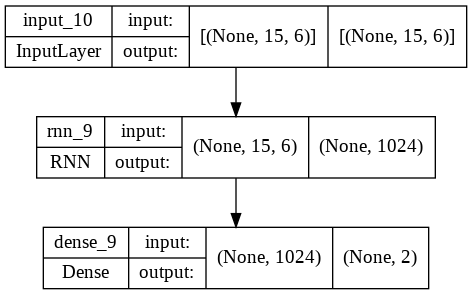
\includegraphics[scale=0.5]{images/q1/elman/architecture.png}
    \caption{معماری شبکه \lr{Elman} در پیاده‌سازی ما}
    \label{elman_architecture}
\end{figure}

در ادامه به تحلیل نتایج حاصل شده می‌پردازیم. نمودار عملکرد مدل در هر گام یادگیری در شکل
\ref{analysing_impact_of_hidden_units_on_elman_network} و نتایج عددی نهایی در جدول \ref{elman_performance_table}
آورده شده است.

\begin{latin}
\begin{table}[!ht]
    \centering
    \caption{\rl{عملکرد شبکه عصبی \lr{Elman} به ازای تعداد نورون‌های مختلف}}
    \label{elman_performance_table}
    \rowcolors{2}{teal!10}{teal!40}
    \begin{tabular}{c|c|c|c|c|c|c|c}
        & & \multicolumn{2}{c|}{\cellcolor{teal!30}train} & \multicolumn{2}{c|}{\cellcolor{teal!30}validation} &  \multicolumn{2}{c}{\cellcolor{teal!30}test} \\ \hline
        index & neurons & loss & accuracy & loss & accuracy & loss & accuracy\\ \hline
        1 & 4 & 0.48 & 0.78 & 0.51 & 0.79 & 0.59 & 0.71 \\
        2 & 16 & 0.41 & 0.80 & 0.45 & 0.77 & 0.49 & 0.74 \\
        3 & 32 & 0.33 & 0.83 & 0.43 & 0.74 & 0.37 & 0.81 \\
        4 & 512 & 0.10 & 0.95 & 0.41 & 0.85 & 0.48 & 0.86 \\
        5 & 1024 & 0.11 & 0.93 & 0.34 & 0.89 & 0.51 & 0.81 \\
    \end{tabular}
\end{table}
\end{latin}

بر طبق انتظار با افزایش نورون‌های لایه مخفی عملکرد مدل رفته‌رفته بهبود می‌یابد، هم از بابت صحت و هم از بابت نرخ \lr{loss}.
با افزایش تعداد نورون‌های لایه مخفی انتظار داشتیم که مدل بر روی داده‌ها دچار پیش‌برازش شود، همان‌طور که در شکل‌ها
مشاهده می‌شود این اتفاق در عمل رخداده است، اما همچنان مدل‌های با تعداد پارامتر بالاتر نسبت به مدل‌های ساده‌تر
عملکرد بهتری دارند. به نظر می‌رسد الگوهای موجود در داده‌ها جزئیات مشترک فراوانی دارند که
با افزایش تعداد نورون‌های لایه مخفی به ۱۰۲۴ مدل همچنان نتایج خوبی را ارائه می‌دهد. با
افزایش تعداد نورون‌های موجود در لایه مخفی جهش‌های فراوانی در عملکرد مدل اتفاق می‌افتد که به نظر می‌رسد با کاهش
نرخ یادگیری بتوان از این اتفاق جلوگیری کرد.

تا این جا به نظر می‌رسد که مدل‌های با تعداد لایه‌های مخفی بیشتر از تمامی جهات بهتر هستند.
باید گفت گر چه صحت عملکرد این مدل‌ها بهتر
است اما این مدل‌ها به علت زیاد بودن تعداد نورون‌های لایه مخفی نسبت به دیگر مدل‌ها در هنگام استنتاج کند‌تر بوده
و زمان بیشتر برای سپری کردن هر گام یادگیری نیاز دارند.

\clearpage

\begin{figure}
    \centering
    \begin{subfigure}{0.45\linewidth}
        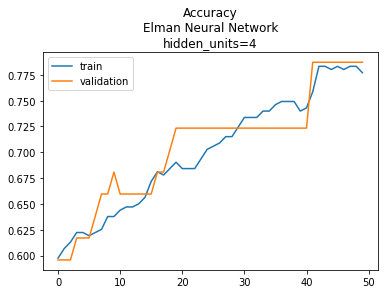
\includegraphics[width=0.9\linewidth]{images/q1/elman/acc_Elman Neural Networkhidden_units=4.png}
    \end{subfigure}
    \hfill
    \begin{subfigure}{0.45\linewidth}
        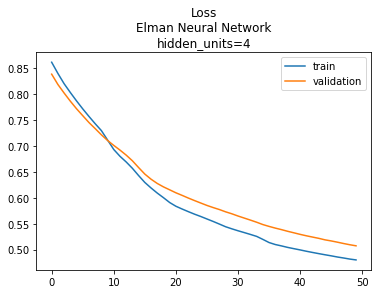
\includegraphics[width=0.9\linewidth]{images/q1/elman/loss_Elman Neural Networkhidden_units=4.png}
    \end{subfigure}
    % \newline
    \begin{subfigure}{0.45\linewidth}
        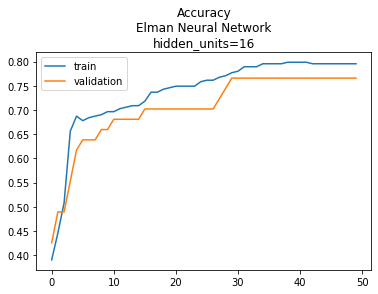
\includegraphics[width=0.9\linewidth]{images/q1/elman/acc_Elman Neural Networkhidden_units=16.png}
    \end{subfigure}
    \hfill
    \begin{subfigure}{0.45\linewidth}
        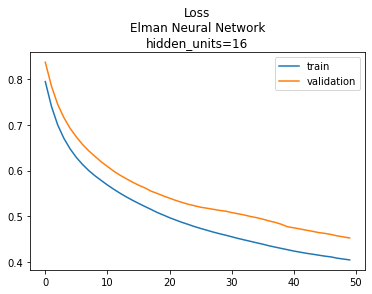
\includegraphics[width=0.9\linewidth]{images/q1/elman/loss_Elman Neural Networkhidden_units=16.png}
    \end{subfigure}
    % /newline
    \begin{subfigure}{0.45\linewidth}
        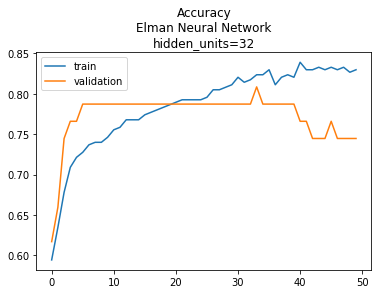
\includegraphics[width=0.9\linewidth]{images/q1/elman/acc_Elman Neural Networkhidden_units=32.png}
    \end{subfigure}
    \hfill
    \begin{subfigure}{0.45\linewidth}
        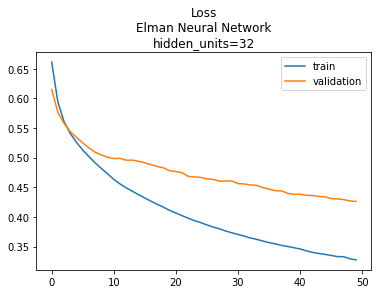
\includegraphics[width=0.9\linewidth]{images/q1/elman/loss_Elman Neural Networkhidden_units=32.png}
    \end{subfigure}
    % \newline
    \begin{subfigure}{0.45\linewidth}
        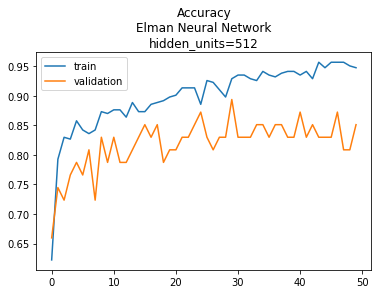
\includegraphics[width=0.9\linewidth]{images/q1/elman/acc_Elman Neural Networkhidden_units=512.png}
    \end{subfigure}
    \hfill
    \begin{subfigure}{0.45\linewidth}
        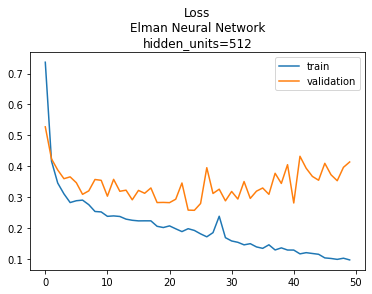
\includegraphics[width=0.9\linewidth]{images/q1/elman/loss_Elman Neural Networkhidden_units=512.png}
    \end{subfigure}
    % /newline
    \begin{subfigure}{0.45\linewidth}
        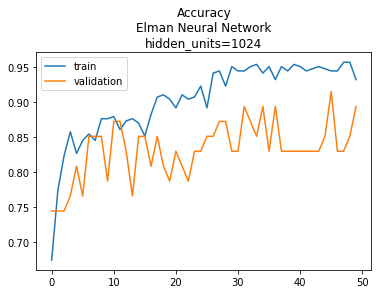
\includegraphics[width=0.9\linewidth]{images/q1/elman/acc_Elman Neural Networkhidden_units=1024.png}
    \end{subfigure}
    \hfill
    \begin{subfigure}{0.45\linewidth}
        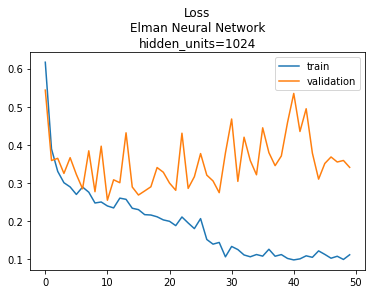
\includegraphics[width=0.9\linewidth]{images/q1/elman/loss_Elman Neural Networkhidden_units=1024.png}
    \end{subfigure}
    \caption{بررسی تاثیر تعداد نورون‌های لایه مخفی بر عملکرد شبکه \lr{Elman}}
    \label{analysing_impact_of_hidden_units_on_elman_network}
\end{figure}

\clearpage

پیش از تحلیل شبکه عصبی \lr{Jordan} ابتدا لازم است توضیحاتی در خصوص جزئیات پیاده‌سازی آن داده شود.
در این شبکه عصبی نیز ما ابتدا یک سلول بازگشتی را با ارث‌بری از کلاس \lr{Layer} توسعه دادیم. با توجه به آن که
در شبکه عصبی \lr{Jordan} خروجی نهایی مدل مجددا به لایه پنهان داده می‌شود، بنابراین در پیاده‌سازی ما لایه \lr{Dense}
در همان سلول انجام شده است. سلول خود دسته خروجی را با استفاده از تابع \lr{softmax} تعیین کرده و مجددا برای تعیین
خروجی بعدی استفاده می‌شود. شکل \ref{jordan_architecture} ساختار پیاده‌سازی انجام شده ما را نشان می‌دهد.

در هنگام آموزش این مدل نیز نرخ یادگیری برابر $10^{-4}$، گام یادگیری برابر ۵۰ و اندازه دسته برابر ۲ در نظر گرفته شده
است.

\begin{figure}[h]
    \centering
    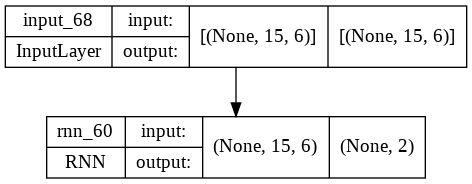
\includegraphics[scale=0.5]{images/q1/jordan/architecture.png}
    \caption{معماری شبکه \lr{Jordan} در پیاده‌سازی ما}
    \label{jordan_architecture}
\end{figure}

حال به بررسی نتایج حاصل شده از این شبکه می‌پردازیم. عملکرد مدل در هر گام یادگیری در شکل
\ref{analysing_impact_of_hidden_units_on_jordan_network} و نتایج نهایی حاصل شده در جدول \ref{jordan_performance_table}
مشاهده می‌شود.

\begin{latin}
\begin{table}[!ht]
    \centering
    \caption{\rl{عملکرد شبکه عصبی \lr{Jordan} به ازای تعداد نورون‌های مختلف}}
    \label{jordan_performance_table}
    \rowcolors{2}{teal!10}{teal!40}
    \begin{tabular}{c|c|c|c|c|c|c|c}
        & & \multicolumn{2}{c|}{\cellcolor{teal!30}train} & \multicolumn{2}{c|}{\cellcolor{teal!30}validation} &  \multicolumn{2}{c}{\cellcolor{teal!30}test} \\ \hline
        index & neurons & loss & accuracy & loss & accuracy & loss & accuracy\\ \hline
        1 & 4 & 0.57 & 0.72 & 0.57 & 0.74 & 0.59 & 0.68 \\
        2 & 16 & 0.48 & 0.77 & 0.50 & 0.81 & 0.48 & 0.74 \\
        3 & 32 & 0.47 & 0.79 & 0.48 & 0.74 & 0.49 & 0.74 \\
        4 & 512 & 0.28 & 0.86 & 0.39 & 0.79 & 0.35 & 0.82 \\
        5 & 1024 & 0.25 & 0.88 & 0.42 & 0.79 & 0.35 & 0.77 \\
    \end{tabular}
\end{table}
\end{latin}

بیشتر تحلیل‌های انجام شده برای نتایج مدل \lr{Elman} در این نتایج نیز دیده می‌شوند. با افزایش تعداد نورون‌های لایه
مخفی نتایج رفته‌رفته بهتر شده است، با افزایش نورون‌ها مدل بر روی نتایج دچار بیش‌پردازش شده اما
همچنان نتایج نهایی نسبت به مدل‌های ساده بهتر است و این که با افزایش
نورون‌ها جهش‌های شدیدی در عملکرد مدل اتفاق می‌افتد. در این شبکه عصبی نیز با افزایش تعداد نورون‌های لایه مخفی
مدل سنگین‌تر شده و زمان بیشتری برای آموزش و استنتاج می‌طلبد.

با مقایسه نتایج حاصل شده از این شبکه عصبی با شبکه عصبی \lr{Elman} مشخص می‌شود عملکرد شبکه عصبی \lr{Elman} نسبت
به شبکه عصبی \lr{Jordan} بهتر است. دلیل این تفاوت عملکرد در ساختار این شبکه‌ها است. در شبکه عصبی \lr{Elman}
خروجی لایه پنهان مجددا توسط همان لایه استفاده می‌شود در حالی که در شبکه عصبی \lr{Jordan} خروجی نهایی شبکه عصبی
مجددا به لایه‌های پنهان داده می‌شود. در این مسئله لایه نهایی \lr{Jordan} دو نورون از نوع \lr{softmax} داشت و
خروجی این دو نورون مجددا توسط نورون‌های لایه مخفی استفاده می‌شد. در حالی که در شبکه عصبی \lr{Elman} خروجی لایه مخفی
که در آزمایش‌های ما حداقل ۴ بود، مجددا به لایه مخفی داده می‌شود. طبیعی است که لایه مخفی با استفاده از خروجی ۴ نورون
بهتر بتواند الگوی داده‌ها را شناسایی کند.

شمای کلی این دو شبکه در شکل \ref{comparison_of_elman_jordan} دیده می‌شود.
همان‌طور که مشاهده می‌شود هر دو این شبکه‌ها از نوع بازگشتی بوده و
از خروجی تولید شده در مراحل قبلی برای تولید خروجی در مرحله فعلی استفاده می‌کنند. تنها تفاوت آن‌ها در خروجی استفاده شده از
مراحل قبلی است. شبکه \lr{Jordan} از خروجی نهایی شبکه در مراحل قبل برای تولید خروجی در مرحله فعلی استفاده می‌کند اما
شبکه \lr{Elman} از خروجی تولید شده توسط لایه پنهان در مرحله قبلی برای تولید خروجی در مرحله فعلی استفاده می‌کند. همین
نکته باعث عملکرد بهتر شبکه عصبی \lr{Elman} نسبت به شبکه عصبی \lr{Jordan} شده است.

\begin{figure}[h]
    \begin{subfigure}{0.5\linewidth}
        \centering
        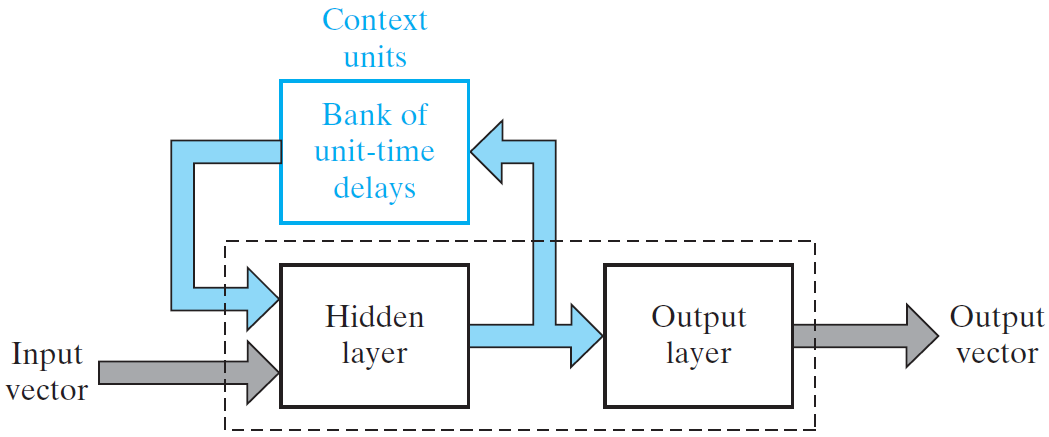
\includegraphics[scale=0.18]{images/q1/elman/schema.png}
        \caption{معماری شبکه \lr{Elman}}
    \end{subfigure}
    \hfill
    \begin{subfigure}{0.5\linewidth}
        \centering
        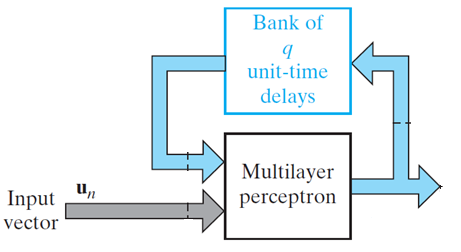
\includegraphics[scale=0.3]{images/q1/jordan/schema.png}
        \caption{معماری شبکه \lr{Jordan}}
    \end{subfigure}
    \caption{مقایسه معماری شبکه‌های \lr{Elman} و \lr{Jordan}}
    \label{comparison_of_elman_jordan}
\end{figure}

در این مسئله دو برچسب را باید پیش‌بینی کنیم. بنابراین آخرین لایه هر دو شبکه دو نورون دارد. شبکه \lr{Jordan}
خروجی همین دو نورون‌ها را به دوباره به شبکه بازگشت می‌دهد، در حالی که شبکه \lr{Elman} خروجی لایه پنهان را به
شبکه بازگشت می‌دهد. بنابراین با افزایش تعداد نورون‌های لایه پنهان شبکه \lr{Elman} تعداد خروجی‌های بیشتری را
به شبکه بازگشت می‌دهد، در حالی که شبکه \lr{Jordan} با افزایش نورون‌ها نیز خروجی همان دو نورون را دوباره به
شبکه بازگشت می‌دهد. به همین دلیل است که شبکه \lr{Elman} در حالت کلی بهتر از شبکه \lr{Jordan} عمل می‌کند.

\clearpage

\begin{figure}
    \centering
    \begin{subfigure}{0.45\linewidth}
        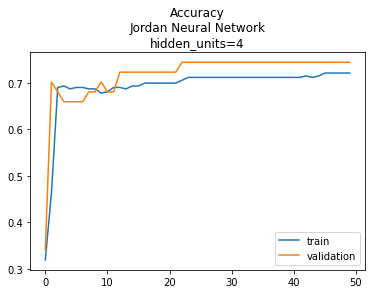
\includegraphics[width=0.9\linewidth]{images/q1/jordan/acc_Jordan Neural Networkhidden_units=4.png}
    \end{subfigure}
    \hfill
    \begin{subfigure}{0.45\linewidth}
        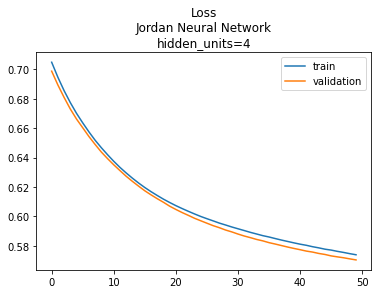
\includegraphics[width=0.9\linewidth]{images/q1/jordan/loss_Jordan Neural Networkhidden_units=4.png}
    \end{subfigure}
    % \newline
    \begin{subfigure}{0.45\linewidth}
        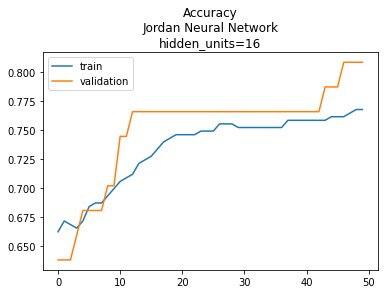
\includegraphics[width=0.9\linewidth]{images/q1/jordan/acc_Jordan Neural Networkhidden_units=16.png}
    \end{subfigure}
    \hfill
    \begin{subfigure}{0.45\linewidth}
        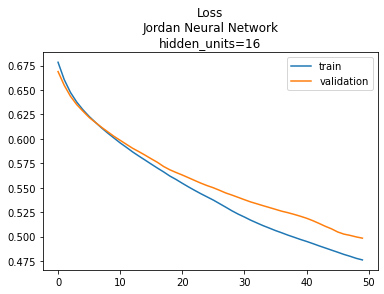
\includegraphics[width=0.9\linewidth]{images/q1/jordan/loss_Jordan Neural Networkhidden_units=16.png}
    \end{subfigure}
    % \newline
    \begin{subfigure}{0.45\linewidth}
        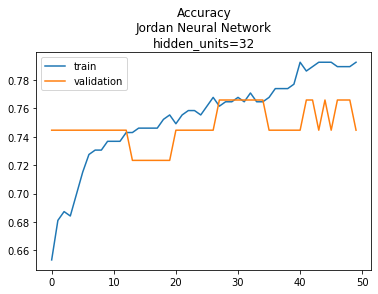
\includegraphics[width=0.9\linewidth]{images/q1/jordan/acc_Jordan Neural Networkhidden_units=32.png}
    \end{subfigure}
    \hfill
    \begin{subfigure}{0.45\linewidth}
        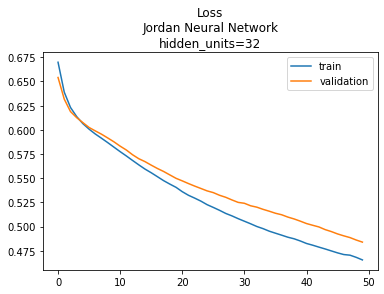
\includegraphics[width=0.9\linewidth]{images/q1/jordan/loss_Jordan Neural Networkhidden_units=32.png}
    \end{subfigure}
    % \newline
    \begin{subfigure}{0.45\linewidth}
        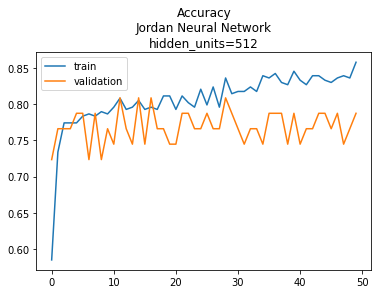
\includegraphics[width=0.9\linewidth]{images/q1/jordan/acc_Jordan Neural Networkhidden_units=512.png}
    \end{subfigure}
    \hfill
    \begin{subfigure}{0.45\linewidth}
        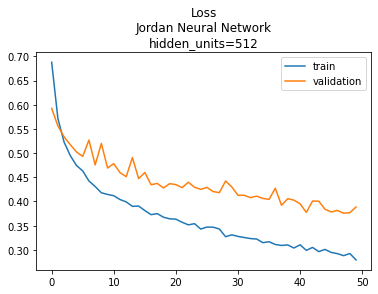
\includegraphics[width=0.9\linewidth]{images/q1/jordan/loss_Jordan Neural Networkhidden_units=512.png}
    \end{subfigure}
    % \newline
    \begin{subfigure}{0.45\linewidth}
        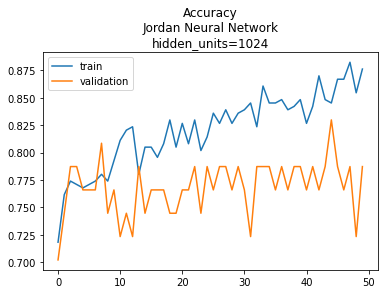
\includegraphics[width=0.9\linewidth]{images/q1/jordan/acc_Jordan Neural Networkhidden_units=1024.png}
    \end{subfigure}
    \hfill
    \begin{subfigure}{0.45\linewidth}
        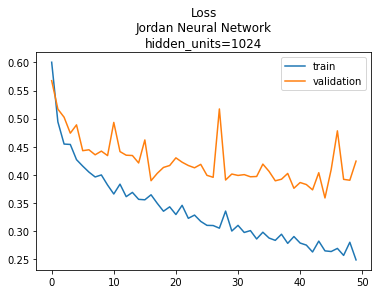
\includegraphics[width=0.9\linewidth]{images/q1/jordan/loss_Jordan Neural Networkhidden_units=1024.png}
    \end{subfigure}
    \caption{بررسی تاثیر تعداد نورون‌های لایه مخفی بر عملکرد شبکه \lr{Jordan}}
    \label{analysing_impact_of_hidden_units_on_jordan_network}
\end{figure}

\clearpage

\section*{سوال دو}

ابتدا توضیحاتی در بابت نحوه پیاده‌سازی مدل‌ ترکیبی می‌دهیم. در مدل ترکیبی ما ورودی به صورت همزمان به همه مدل‌ها
داده شده و مدل‌ها خروجی مد نظر خود را تولید می‌کنند. تمامی خروجی‌های تولید شده توسط این زیرمدل‌ها در مرحله بعد به یک
لایه میانگین‌گیر داده می‌شود. خروجی همین لایه میانگین‌گیر به عنوان خروجی نهایی مدل در نظر گرفته می‌شود.
بدین ترتیب خود مدل به غیر از آموزش زیرمدل‌ها پارامتر دیگری برای آموزش ندارد.

آموزش زیر شبکه‌ها نیز مطابق روال طی شده در سوال قبلی آموزش داده می‌شود. پارامتر‌های در نظر گرفته شده در هنگام
آموزش نیز همان پارامتر‌ها بوده و تغییری داده نشده است. در ادامه به بررسی تاثیر تجمیع این شبکه‌ها با هم می‌پردازیم.

\subsection*{هنگامی که مجموعه داده بین زیرمدل‌ها مشترک است.}

در جداول \ref{pure_elman_performance_common_dataset}، \ref{pure_jordan_performance_common_dataset}
و \ref{elman_jordan_performance_common_dataset} عملکرد مدل‌ها در هنگامی که داده‌ آموزشی زیرمدل‌ها یکسان است مشاهده می‌شود.
با مقایسه این نتایج با نتایج حاصل از عملکرد مدل‌ها در حالت تکی مشاهده می‌شود که عملکرد مدل‌ها در حالت ترکیب شبکه‌های
\lr{Elman} نسبت به حالت‌های تکی بهبود چندانی نداشته است. اما در حالت ترکیب شبکه‌های \lr{Jordan} عملکرد مدل
ترکیبی نسبت به تک شبکه‌های \lr{Jordan} بهبود داشته است. در مدل‌های ترکیبی \lr{Elman} و \lr{Jordan} عملکرد شبکه نسبت
به تک شبکه \lr{Jordan} بهتر است اما تغییر چندانی نسبت به تک شبکه‌های \lr{Elman} ندارد.

علت این که مدل ترکیبی \lr{Elman} نسبت به تک شبکه‌های \lr{Elman} بهبود آنچنانی نداشته را می‌توان در این
دانست که مدل \lr{Elman} در حالت‌های ساده خود به اندازه کافی پیچیده است در نتیجه با ترکیب این شبکه‌ها نمی‌توان
به دقت‌های بالایی رسید. اما ترکیب کردن شبکه‌ها باعث شده است مقدار \lr{loss} به صورت کلی کم شود. علت این رخداد
آن است که هر یک از شبکه‌ها به صورت مجزا از یکدیگر روی داده‌ آموزش دیده‌اند. بنابراین با ترکیب این شبکه‌ها
مدل نهایی می‌تواند با تجمیع این دانش‌ها با دقت بهتری احتمال متعلق بودن به هر کلاس را به دست آورد.

\begin{latin}
\begin{table}[h]
    \centering
    \caption{\rl{نتایج شبکه عصبی با ترکیب شبکه‌های \lr{Elman}}}
    \label{pure_elman_performance_common_dataset}
    \rowcolors{2}{teal!10}{teal!40}
    \begin{tabular}{c|p{3cm}|c|c|c|c|c|c}
        & & \multicolumn{2}{c|}{\cellcolor{teal!30}train} & \multicolumn{2}{c|}{\cellcolor{teal!30}validation} &  \multicolumn{2}{c}{\cellcolor{teal!30}test} \\ \hline
        index & description & loss & accuracy & loss & accuracy & loss & accuracy\\ \hline
        1 & 5 * Elman(4) & 0.47 & 0.74 & 0.51 & 0.77 & 0.56 & 0.68 \\
        2 & 5 * Elman(32) & 0.20 & 0.92 & 0.30 & 0.81 & 0.36 & 0.77 \\
        3 & 5 * Elman(1024) & 0.06 & 0.97 & 0.80 & 0.85 & 1.00 & 0.82 \\
        4 & Elman(4) + Elman(1024) & 0.25 & 0.96 & 0.38 & 0.85 & 0.41 & 0.83 \\
        5 & Elman(4) + Elman(16) + Elman(32) + Elman(512) + Elman(1024) & 0.27 & 0.96 & 0.38 & 0.89 & 0.40 & 0.82 \\
    \end{tabular}
\end{table}
\end{latin}

همان‌طور که بیان شد مدل حاصل از ترکیب شبکه‌های \lr{Jordan} نسبت به حالت عادی شبکه‌های \lr{Jordan} بهتر عمل می‌کند.
چرا که مدل‌های \lr{Jordan} به صورت تکی نمی‌توانست همه دانش را به خوبی در خود نگه دارد، اما ترکیب این شبکه‌ها
بهتر می‌تواند دانش کلی داده‌ها را در خود ذخیره کند. هر مدل به صورت جداگانه آموزش دیده و دارای دانش کوچکی از
داده‌ها است. با ترکیب دانش این مدل‌های کوچک می‌توانند عملکرد بهتری را نشان دهند. در این جا نیز همان‌طور که در جدول
\ref{pure_jordan_performance_common_dataset} دیده می‌شود، شبکه‌ها هم از نظر معیار \lr{accuracy} و هم از نظر
معیار \lr{loss} بهبود داشته‌اند.

\begin{latin}
\begin{table}[h]
    \centering
    \caption{\rl{نتایج شبکه عصبی با ترکیب شبکه‌های \lr{Jordan}}}
    \label{pure_jordan_performance_common_dataset}
    \rowcolors{2}{teal!10}{teal!40}
    \begin{tabular}{c|p{3cm}|c|c|c|c|c|c}
        & & \multicolumn{2}{c|}{\cellcolor{teal!30}train} & \multicolumn{2}{c|}{\cellcolor{teal!30}validation} &  \multicolumn{2}{c}{\cellcolor{teal!30}test} \\ \hline
        index & description & loss & accuracy & loss & accuracy & loss & accuracy\\ \hline
        1 & 5 * Jordan(4) & 0.48 & 0.81 & 0.49 & 0.81 & 0.55 & 0.74 \\ \hline
        2 & 5 * Jordan(32) & 0.28 & 0.86 & 0.39 & 0.77 & 0.35 & 0.83 \\ \hline
        3 & 5 * Jordan(1024) & 0.14 & 0.94 & 0.31 & 0.85 & 0.40 & 0.83 \\ \hline
        4 & Jordan(4) + Jordan(1024) & 0.40 & 0.83 & 0.45 & 0.81 & 0.44 & 0.80 \\ \hline
        5 & Jordan(4) + Jordan(16) + Jordan(32) + Jordan(512) + Jordan(1024) & 0.38 & 0.84 & 0.43 & 0.79 & 0.42 & 0.78 \\ \hline
     \end{tabular}
\end{table}
\end{latin}

عملکرد مدل ترکیبی از \lr{Elman} و \lr{Jordan} مابین مدل‌های تکی قرار می‌گیرد.
به نوعی می‌توان گفت که در این مدل، شبکه‌های \lr{Elman} به بهبود نتیجه کمک می‌کنند
اما مدل‌های \lr{Jordan} با توجه به عملکرد بد آن‌ها در حالت عادی، باعث افت عملکرد مدل می‌شوند.

\begin{latin}
\begin{table}[h]
    \centering
    \caption{\rl{نتایج شبکه عصبی با ترکیب شبکه‌های \lr{Jordan} و \lr{Elman}}}
    \label{elman_jordan_performance_common_dataset}
    \rowcolors{2}{teal!10}{teal!40}
    \begin{tabular}{c|p{3cm}|c|c|c|c|c|c}
        & & \multicolumn{2}{c|}{\cellcolor{teal!30}train} & \multicolumn{2}{c|}{\cellcolor{teal!30}validation} &  \multicolumn{2}{c}{\cellcolor{teal!30}test} \\ \hline
        index & description & loss & accuracy & loss & accuracy & loss & accuracy\\ \hline
        1 & 2 * Elman(4) + 2 * Jordan(4) & 0.52 & 0.77 & 0.53 & 0.77 & 0.54 & 0.76 \\ \hline
        2 & 2 * Elman(32) + 2 * Jordan (32) & 0.36 & 0.80 & 0.40 & 0.74 & 0.46 & 0.75 \\ \hline
        3 & 2 * Elman(1024) + 2 * Jordan (1024) & 0.15 & 0.95 & 0.30 & 0.89 & 0.35 & 0.84 \\ \hline
        4 & Elman(4) + Elman(1024) + Jordan(4) + Jordan (1024) & 0.32 & 0.93 & 0.39 & 0.79 & 0.42 & 0.85
    \end{tabular}
\end{table}
\end{latin}

\subsection*{هنگامی که مجموعه داده بین زیرمدل‌ها متفاوت است.}

نتایج این حالت در جدول‌های \ref{pure_elman_performance_different_dataset}، \ref{pure_jordan_performance_different_dataset}
و \ref{elman_jordan_performance_different_dataset} دیده می‌شود. همان‌طور که مشاهده می‌شود نتایج مدل نسبت به حالت
قبل بدتر شده است. دلیل این افت عملکرد را می‌توان در تعداد محدود مجموعه داده آموزشی برای آموزش هر زیرشبکه دانست.
تعداد کل داده‌های آموزشی شبکه حدود ۳۰۰تاست. با پخش کردن این تعداد داده‌های آموزشی بین ۵ زیرشبکه مختلف تقسیم کنیم
برای هر شبکه ۶۰ داده آموزشی می‌ماند که تعداد بسیار کمی برای آموزش یک شبکه عصبی است.

\begin{latin}
\begin{table}[h]
    \centering
    \caption{\rl{نتایج شبکه عصبی با ترکیب شبکه‌های \lr{Elman}}}
    \label{pure_elman_performance_different_dataset}
    \rowcolors{2}{teal!10}{teal!40}
    \begin{tabular}{c|p{3cm}|c|c|c|c|c|c}
        & & \multicolumn{2}{c|}{\cellcolor{teal!30}train} & \multicolumn{2}{c|}{\cellcolor{teal!30}validation} &  \multicolumn{2}{c}{\cellcolor{teal!30}test} \\ \hline
        index & description & loss & accuracy & loss & accuracy & loss & accuracy\\ \hline
        1 & 5 * Elman(4) & 0.60 & 0.67 & 0.61 & 0.66 & 0.58 & 0.70 \\
        2 & 5 * Elman(32) & 0.51 & 0.77 & 0.52 & 0.74 & 0.51 & 0.77 \\
        3 & 5 * Elman(1024) & 0.36 & 0.83 & 0.38 & 0.77 & 0.44 & 0.75 \\
        4 & Elman(4) + Elman(1024) & 0.39 & 0.87 & 0.40 & 0.81 & 0.44 & 0.84 \\
        5 & Elman(4) + Elman(16), Elman(32), Elman(512), Elman(1024) & 0.48 & 0.78 & 0.47 & 0.74 & 0.49 & 0.82 \\
     \end{tabular}
\end{table}
\end{latin}

\begin{latin}
\begin{table}[h]
    \centering
    \caption{\rl{نتایج شبکه عصبی با ترکیب شبکه‌های \lr{Jordan}}}
    \label{pure_jordan_performance_different_dataset}
    \rowcolors{2}{teal!10}{teal!40}
    \begin{tabular}{c|p{3cm}|c|c|c|c|c|c}
        & & \multicolumn{2}{c|}{\cellcolor{teal!30}train} & \multicolumn{2}{c|}{\cellcolor{teal!30}validation} &  \multicolumn{2}{c}{\cellcolor{teal!30}test} \\ \hline
        index & description & loss & accuracy & loss & accuracy & loss & accuracy\\ \hline
        1 & 5 * Jordan(4) & 0.64 & 0.67 & 0.65 & 0.66 & 0.64 & 0.70 \\
        2 & 5 * Jordan(32) & 0.64 & 0.70 & 0.64 & 0.68 & 0.64 & 0.74 \\
        3 & 5 * Jordan(1024) & 0.65 & 0.70 & 0.65 & 0.66 & 0.64 & 0.73 \\
        4 & Jordan(4) + Jordan(1024) & 0.44 & 0.80 & 0.48 & 0.81 & 0.50 & 0.76 \\
        5 & Jordan(4) + Jordan(16) + Jordan(32) + Jordan(512) + Jordan(1024) & 0.65 & 0.68 & 0.65 & 0.66 & 0.65 & 0.72 \\
    \end{tabular}
\end{table}
\end{latin}

\clearpage

\begin{latin}
\begin{table}[h]
    \centering
    \caption{\rl{نتایج شبکه عصبی با ترکیب شبکه‌های \lr{Jordan} و \lr{Elman}}}
    \label{elman_jordan_performance_different_dataset}
    \rowcolors{2}{teal!10}{teal!40}
    \begin{tabular}{c|p{3cm}|c|c|c|c|c|c}
        & & \multicolumn{2}{c|}{\cellcolor{teal!30}train} & \multicolumn{2}{c|}{\cellcolor{teal!30}validation} &  \multicolumn{2}{c}{\cellcolor{teal!30}test} \\ \hline
        index & description & loss & accuracy & loss & accuracy & loss & accuracy\\ \hline
        1 & 2 * Elman(4) + 2 * Jordan(4) & 0.60 & 0.71 & 0.63 & 0.68 & 0.60 & 0.72 \\
        2 & 2 * Elman(32) + 2 * Jordan (32) & 0.53 & 0.77 & 0.57 & 0.70 & 0.55 & 0.76 \\
        3 & 2 * Elman(1024) + 2 * Jordan (1024) & 0.34 & 0.85 & 0.40 & 0.79 & 0.44 & 0.76 \\
        4 & Elman(4) + Elman(1024) + Jordan(4) + Jordan(1024) & 0.48 & 0.82 & 0.51 & 0.74 & 0.50 & 0.77 \\
        5 & 3 * Elman(32) + 2 * Jordan(1024) & 0.46 & 0.79 & 0.48 & 0.70 & 0.50 & 0.78
    \end{tabular}
\end{table}
\end{latin}

برای بررسی تاثیر تعداد زیرشبکه‌ها بر روی عملکرد کلی مدل تجمیع شده شبکه‌های عصبی \lr{Elman} و \lr{Jordan} را
با ۳۲ لایه پنهان را امتحان می‌کنیم. نتایج این مدل در جدول \ref{analysing_impact_of_number_of_subnetwork_elman}
و \ref{analysing_impact_of_number_of_subnetwork_jordan} آورده شده است. با افزایش تعداد زیر شبکه‌ها همان‌طور که
در قسمت‌های قبل دیدیم عملکرد کلی مدل بهتر می‌شود اما در این جا چون داده‌های آموزشی بین زیرشبکه‌ها افراز شده است
بنابراین با افزایش تعداد زیرمدل‌ها تعداد داده آموزشی که هر مدل در اختیار دارد کم‌تر می‌شود. بنابراین هر مدل
نمی‌تواند به خوبی الگوی داده‌ها را آموخته و در نتیجه مدل عملکرد ضعیف‌تری را از خود نشان می‌دهد.

\begin{latin}
\begin{table}[!ht]
    \centering
    \caption{\rl{عملکرد شبکه عصبی تجمیع شده با تعداد مختلف زیرشبکه \lr{Elman}}}
    \label{analysing_impact_of_number_of_subnetwork_elman}
    \rowcolors{2}{teal!10}{teal!40}
    \begin{tabular}{c|p{3cm}|c|c|c|c|c|c}
        & & \multicolumn{2}{c|}{\cellcolor{teal!30}train} & \multicolumn{2}{c|}{\cellcolor{teal!30}validation} &  \multicolumn{2}{c}{\cellcolor{teal!30}test} \\ \hline
        index & description & loss & accuracy & loss & accuracy & loss & accuracy\\ \hline
        1 & Elmant(32) & 0.33 & 0.83 & 0.43 & 0.74 & 0.37 & 0.81 \\
        2 & 2 * Elman(32) & 0.38 & 0.81 & 0.43 & 0.72 & 0.49 & 0.74 \\
        3 & 4 * Elman(32) & 0.46 & 0.77 & 0.52 & 0.70 & 0.54 & 0.75 \\
        4 & 8 * Elman(32) & 0.54 & 0.74 & 0.56 & 0.70 & 0.58 & 0.73 \\
        5 & 16 * Elman(32) & 0.59 & 0.72 & 0.60 & 0.68 & 0.60 & 0.72 \\
    \end{tabular}
\end{table}
\end{latin}

\clearpage

\begin{latin}
\begin{table}[!ht]
    \centering
    \caption{\rl{عملکرد شبکه عصبی تجمیع شده با تعداد مختلف زیرشبکه \lr{Jordan}}}
    \label{analysing_impact_of_number_of_subnetwork_jordan}
    \rowcolors{2}{teal!10}{teal!40}
    \begin{tabular}{c|p{3cm}|c|c|c|c|c|c}
        & & \multicolumn{2}{c|}{\cellcolor{teal!30}train} & \multicolumn{2}{c|}{\cellcolor{teal!30}validation} &  \multicolumn{2}{c}{\cellcolor{teal!30}test} \\ \hline
        index & description & loss & accuracy & loss & accuracy & loss & accuracy\\ \hline
        1 & Jordan(32) & 0.47 & 0.79 & 0.48 & 0.74 & 0.49 & 0.74 \\
        2 & 2 * Jordan(32) & 0.50 & 0.77 & 0.55 & 0.70 & 0.56 & 0.72 \\ \hline
        3 & 4 * Jordan(32) & 0.55 & 0.75 & 0.58 & 0.68 & 0.57 & 0.73 \\ \hline
        4 & 8 * Jordan(32) & 0.59 & 0.72 & 0.60 & 0.68 & 0.59 & 0.75 \\ \hline
        5 & 16 * Jordan(32) & 0.62 & 0.70 & 0.63 & 0.68 & 0.61 & 0.75 \\ \hline
     \end{tabular}
\end{table}
\end{latin}


\end{document}